\documentclass[]{article}

\usepackage[utf8]{inputenc}
\usepackage{listings}
\usepackage{color}
\usepackage[french]{babel}
\usepackage[all]{xy} % color,matrix,arrow

%\definecolor{lightgray}{rgb}{.9,.9,.9}
%\definecolor{darkgray}{rgb}{.4,.4,.4}
%\definecolor{purple}{rgb}{0.65, 0.12, 0.82}

%\lstdefinelanguage{JavaScript}{
%	keywords={typeof, new, true, false, catch, function, return, null, catch, switch, var, if, in, while, do, else, case, break, const},
%	keywordstyle=\color{blue}\bfseries,
%	ndkeywords={class, export, boolean, throw, implements, import, this},
%	ndkeywordstyle=\color{darkgray}\bfseries,
%	identifierstyle=\color{black},
%	sensitive=false,
%	comment=[l]{//},
%	morecomment=[s]{/*}{*/},
%	commentstyle=\color{purple}\ttfamily,
%	stringstyle=\color{red}\ttfamily,
%	morestring=[b]',
%	morestring=[b]"
%}
%\lstset{
%	language=JavaScript,
%	backgroundcolor=\color{lightgray},
%	extendedchars=true,
%	basicstyle=\footnotesize\ttfamily,
%	showstringspaces=false,
%	showspaces=false,
%	numbers=left,
%	numberstyle=\footnotesize,
%	numbersep=9pt,
%	tabsize=2,
%	breaklines=true,
%	showtabs=false,
%	captionpos=b
%}

\usepackage{amsmath}

\usepackage[left=2cm, right=2cm, top=2cm]{geometry}
\usepackage{multicol}
%\setlength{\columnseprule}{.1pt}
\usepackage{tabularx}

\usepackage{graphicx}
\graphicspath{{./medias/}}

\title{Implantation fonctionnelle d'algorithmes géométriques en 3D}
\author{Titouan Laurent}
\date{}

\begin{document}

\maketitle

\begin{multicols}{2}

\section{Introduction}
\section{Structures de données implémentées}

\subsection{Données d'entrées}
Un $vec3$ permet de modéliser aussi bien un point qu'un vecteur dans l'espace 3D. Les composantes sont données dans l'ordre usuel $x$, $y$ et $z$ ($x, y, z \in \mathbf{R}$).\\
Dans notre implémentation, on considérera une simple liste ordonnée des $n$ points (sous le nom de la variable globale $GLOBAL\_V\_LIST$) représentant les données d'entrée du problème à résoudre.\\

\subsection{Stockage et manipulation de l'enveloppe convexe en mémoire}
La structure en liste de demi-arêtes orientées (doubly connected edge list, abrégé DCEL) est parmi les plus communes qu'il soit dès lors que l'on souhaite modéliser un maillage topologique.\\\\
Ici on implante une version plus limitée de cette dernière, puisqu'elle permet de créer maillages triangulaires uniquement — ce qui est sans effet sur les capacités du programme final.

\subsubsection{Demi-arête — $he$}
Une $he$ (abrévation de halfedge, ou demi-arête) est une structure de données disposant d'informations sur elle-même et son voisinage topologique. Celles-ci sont les suivantes :
\begin{itemize}
	\item $index \in \mathbf{Z}$, un identifiant unique pour la demi-arête, avec :
		\[
			\left\{
				\begin{array}{ll}
					index = -1		& \mbox{est une demi-arête nulle} \\
					index \geq 0 	& \mbox{sinon}
				\end{array}
			\right.
		\]
	\item $opposite \in \mathbf{Z}$, l'identifiant de la demi-arête opposée, avec :
		\[
			\left\{
				\begin{array}{ll}
					opposite = -1 		& \text{est une demi-arête du bord} \\
					opposite \geq 0 	& \text{sinon}
				\end{array}
			\right.
		\]
	\item $vertex \in \mathbf{N}$, l'indice du sommet incident dont elle est issue.
\end{itemize}

\subsubsection{Maillage triangulaire — $dcel$}
Une $dcel$ permet la modélisation d'un maillage topologique triangulaire. Elle dispose des attributs suivants :
\begin{itemize}
	\item $he\_list$, une liste de $he$.
	\item $available\_he\_index \in \mathbf{N}$, le prochain indice non attribué à une $he$ de la liste.
\end{itemize}

\subsubsection{Exemple simple en 2D}

	\begin{figure}[!h]
		\[
	\begin{aligned}[c]
		\entrymodifiers={+[o][F]}
		\renewcommand{\labelstyle}{\textstyle}
		\xymatrix@=4em @L=.25ex{
			{}
			\ar @^{-} [d]
			\ar @^{-} [dr]
			& {}
			\ar @^{-} [l]
			\\ {}
			\ar @^{-} [r]
			& {}
			\ar @^{-} [u]
		}
	\end{aligned}
	\rightarrow
	\begin{aligned}[c]
		\entrymodifiers={+[o][F]}
		\renewcommand{\labelstyle}{\textstyle}
		\xymatrix@=4em @L=.25ex{
			{\color{red}0}
			\ar @<.25ex> @^{->} [d] |{\color{blue}0}
			\ar @<.25ex> @^{->} [dr] ^{\color{blue}4}
			& {\color{red}1}
			\ar @<.25ex> @^{->} [l] |{\color{blue}3}
			\\ {\color{red}2}
			\ar @<.25ex> @^{->} [r] |{\color{blue}1}
			& {\color{red}3}
			\ar @<.25ex> @^{->} [ul] ^{\color{blue}2}
			\ar @<.25ex> @^{->} [u] |{\color{blue}5}
		}
	\end{aligned}
		\]
		\caption{Un maillage simple et un indiçage correspondant possible.}
		\label{maillage_simple}
	\end{figure}

%	\begin{figure}[!h]
%		\begin{aligned}[c]
%			\begin{array}{l}
%				\begin{tabular}{|c|c|c|c|}
%					\hline
%					index & opposite & vertex \\
%					\hline
%					\color{blue}0 & -1 & \color{red}0 \\
%					\hline
%					\color{blue}1 & -1 & \color{red}2 \\
%					\hline
%					\color{blue}2 & \color{blue}4 & \color{red}3 \\
%					\hline
%					\color{blue}3 & -1 & \color{red}1 \\
%					\hline
%					\color{blue}4 & \color{blue}2 & \color{red}0 \\
%					\hline
%					\color{blue}5 & -1 & \color{red}3 \\
%					\hline
%				\end{tabular}\\\\
%				available\_he\_index\textbf{ : }6
%			\end{array}
%		\end{aligned}
%		\begin{aligned}[c]
%			\begin{tabular}{|c|c|}
%				\hline
%				Indice & Coordonnées \\
%				\hline
%				\color{red}0 & (0,0) \\
%				\hline
%				\color{red}1 & (1,0) \\
%				\hline
%				\color{red}2 & (1,1) \\
%				\hline
%				\color{red}3 & (0,1) \\
%				\hline
%			\end{tabular}
%		\end{aligned}
%		\]
%		\caption{Structure DCEL à gauche et table des sommets à droite.}
%		\label{maillage_simple_struct_associee}
%	\end{figure}

	Considérons le maillage de la Figure~\ref{maillage_simple}. Une structure $dcel$ associée valide serait alors telle que celle présentée Figure~\ref{maillage_simple_struct_associee}.\\\\
	Note : si les numéros d'indices choisis pour les demi-arêtes sont plus ou moins arbitraires, la structure $dcel$ impose tout de même des contraintes comme nous allons le voir.
	
	
	\subsubsection{Ajout et retrait d'une face dans une $dcel$}
	Les opérations de modification d'une $dcel$ sont au nombre de deux (si l'on ne prend pas en compte le constructeur) : l'ajout et le retrait de face.\\\\
	L'ajout d'une nouvelle face entraine implicitement la création de trois demi-arêtes ($he$) dans la structure. Leur indice est lui calculé aux lignes 3, 4 et 5. De même, l'indice de leur demi-arête opposée respective (si elle existe) est recherché parmi toutes les demi-arêtes de $dcel$ aux lignes 7, 8 et 9.
	Notez que l'attribut $dcel.available\_he\_index$ est mis à jour dans la structure retournée ligne 29.
%	\begin{lstlisting}
%	const add_face = (dcel, vert_A, vert_B, vert_C) =>
%	{
%		const he_AB_index = dcel.available_he_index;
%		const he_BC_index = dcel.available_he_index + 1;
%		const he_CA_index = dcel.available_he_index + 2;
%		
%		const he_AB_opposite_index = look_up_for_opposite_he_index(dcel, vert_A, vert_B);
%		const he_BC_opposite_index = look_up_for_opposite_he_index(dcel, vert_B, vert_C);
%		const he_CA_opposite_index = look_up_for_opposite_he_index(dcel, vert_C, vert_A);
%		
%		return new_dcel(
%			dcel.he_list.map((current_he) =>
%			{
%				switch(he_index(current_he))
%				{
%					case he_AB_opposite_index:
%						return set_he_opposite(current_he, he_AB_index);
%					case he_BC_opposite_index:
%						return set_he_opposite(current_he, he_BC_index);
%					case he_CA_opposite_index:
%						return set_he_opposite(current_he, he_CA_index);
%				}
%				return current_he;
%			})
%			.concat(new_he(he_AB_index, he_AB_opposite_index, vert_A))
%			.concat(new_he(he_BC_index, he_BC_opposite_index, vert_B))
%			.concat(new_he(he_CA_index, he_CA_opposite_index, vert_C)),
%			dcel.available_he_index + 3
%		);
%	};
%	\end{lstlisting}
	
\section{Évaluation des performances}

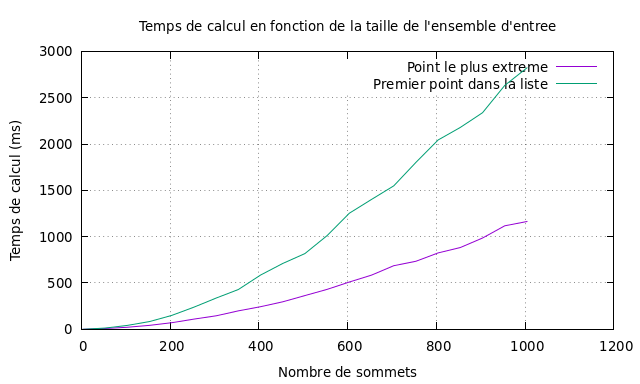
\includegraphics[scale=.5]{perf_extreme.png}

\end{multicols}{2}

\end{document}